%%%%%%%%%%%%%%%%%%%%%%%%%%%%%%%%%%%%%%%%%%%%%%%%%%%%%%%%%%%%%%%%%%%%%%
% LaTeX Example: Project Report
%
% Source: http://www.howtotex.com
%
% Feel free to distribute this example, but please keep the referral
% to howtotex.com
% Date: March 2011 
% 
%%%%%%%%%%%%%%%%%%%%%%%%%%%%%%%%%%%%%%%%%%%%%%%%%%%%%%%%%%%%%%%%%%%%%%
% How to use writeLaTeX: 
%
% You edit the source code here on the left, and the preview on the
% right shows you the result within a few seconds.
%
% Bookmark this page and share the URL with your co-authors. They can
% edit at the same time!
%
% You can upload figures, bibliographies, custom classes and
% styles using the files menu.
%
% If you're new to LaTeX, the wikibook is a great place to start:
% http://en.wikibooks.org/wiki/LaTeX
%
%%%%%%%%%%%%%%%%%%%%%%%%%%%%%%%%%%%%%%%%%%%%%%%%%%%%%%%%%%%%%%%%%%%%%%
% Edit the title below to update the display in My Documents
%\title{Project Report}
%
%%% Preamble
\documentclass[paper=a4, fontsize=11pt]{scrartcl}
\usepackage[T1]{fontenc}
\usepackage{fourier}
\usepackage[english]{babel}			 % English language/hyphenation												
\usepackage[protrusion=true,expansion=true]{microtype}	
\usepackage{amsmath,amsfonts,amsthm} % Math packages
\usepackage[pdftex]{graphicx}	
\usepackage{url}

\usepackage{sectsty}   %%% Custom sectioning
\allsectionsfont{\centering \normalfont\scshape}


%%% Custom headers/footers (fancyhdr package)
\usepackage{fancyhdr}
\pagestyle{fancyplain}
\fancyhead{}											% No page header
\fancyfoot[L]{}											% Empty 
\fancyfoot[C]{}											% Empty
\fancyfoot[R]{\thepage}									% Pagenumbering
\renewcommand{\headrulewidth}{0pt}			% Remove header underlines
\renewcommand{\footrulewidth}{0pt}				% Remove footer underlines
\setlength{\headheight}{13.6pt}


%%% Equation and float numbering
\numberwithin{equation}{section}		% Equationnumbering: section.eq#
\numberwithin{figure}{section}			% Figurenumbering: section.fig#
\numberwithin{table}{section}				% Tablenumbering: section.tab#


%%% Maketitle metadata
\newcommand{\horrule}[1]{\rule{\linewidth}{#1}} 	% Horizontal rule

\title{
		%\vspace{-1in} 	
		\usefont{OT1}{bch}{b}{n}
		\normalfont \normalsize \textsc{School of Computer Science} \\ 
        \normalsize \textsc{High Performance Architecture (COMPSCI 243)} \\
        [25pt]
		\horrule{0.5pt} \\[0.4cm]
		\huge GPU Benchmarking Report \\
		\horrule{2pt} \\[0.5cm]
}
\author{
		\normalfont 								
        \normalsize
        Zahra Montazeri (ID??) \\[-3pt]		
        \normalsize 
        \newline
        \normalsize
        Nitin Agarwal (84246130) \\[-3pt]		
        \normalsize 
        \newline
        \newline
        \today
}
\date{}
\newpage

%%% Begin document
\begin{document}
\maketitle
\newpage
\tableofcontents
\newpage
\section{Vision and Scope}
In this project, a set of well-defined test cases for GPU have been used to compare the performances of different graphics cards across differnt platforms. The main focus of the project has been to use the various test cases with similar settings on multiple graphics cards, keeping everything else the same. We perform benchmarking on three different NVIDIA Graphic Cards and profile the test cases using an NVIDIA profiler \textbf{nvprof}. We show the results of each of the test cases and further perform analysis.\\

The project involved searching of well-known, published test cases, which could be tested on Linux platforms. All benchmarks have been performed using the release 3.1 version of the Rodinia \ref{•}. Several test cases from Rodinia were profiled using nvprof (NVIDIA profiling tool), which is a command-line profiler available for Linux, Windows, and OS X. It helps users to understand and optimize the performance of cuda applications and easily compare and analyze the result of benchmarks on different GPUs. A cuda version of 7.5 was used to benchmark all three graphic cards in this project. The three NVIDIA graphics cards benchmarked are GTX 630, GTX 650 \& Quadro M6000.\\

We chose seven different test cases and profiled several parameters for each test case. We compare and analyze these values across all three different GPU cards. We profiled the following parameters:

\begin{itemize}
\item
\textit{Total time for all API calls: } explanation??

\item
\textit{Total time for all Kernel calls: } explanation??

\item
\textit{Number of registers per thread for each Kernel call: } explanation?

\item
\textit{Temperature: } We understand that temperature and fan-speed would be more relevant in for benchmarking mobile GPU's, but for completeness we profiled them both.

\item
\textit{Fan Speed: }
\end{itemize}



\newpage
\section{Description of Benchmarks}
This section provides a brief description of all the seven test cases used 
to benchmark the three NVIDIA GPU cards.

\subsection{Breadth First Search}
Graph algorithms are fundamental and widely used in many disciplines and application areas. Large graphs involving millions of vertices are common in scientific and engineering applications. This benchmark suite provides the GPU implementations of breadth-first search (BFS) algorithm which traverses all the connected components in a graph.

\subsection{K-Nearest Neighbor}
NN (Nearest Neighbor) finds the k-nearest neighbors from an unstructured data set. The sequential NN algorithm reads in one record at a time, calculates the Euclidean distance from the target latitude and longitude, and evaluates the k nearest neighbors. The parallel versions read in many records at a time, execute the distance calculation on multiple threads, and the master thread updates the list of nearest neighbors.

\subsection{B+Tree}
B+ Tree application has many internal commands that maintain database and process querries. Only J and K commands had enough parallelism to be ported to parallel languages (OpenMP, CUDA, OpenCL). In these implementations, in case of both J and K, the same algorithms (optimized for exposing fine-grained parallelism) were used for fair comparison purposes. For C/OpenMP execution, it is possible to use the original algorithm.

\subsection{PathFinder}
PathFinder uses dynamic programming to find a path on a 2-D grid from the bottom row to the top row with the smallest accumulated weights, where each step of the path moves straight ahead or diagonally ahead. It iterates row by row, each node picks a neighboring node in the previous row that has the smallest accu- mulated weight, and adds its own weight to the sum.
This kernel uses the technique of ghost zone optimization.

\subsection{LU Decomposition}
LU Decomposition is an algorithm to calculate the solutions of a set of linear equations. The LUD kernel decomposes a matrix as the product of a lower triangular matrix and an upper triangular matrix.

\subsection{Gaussian Elimination}
Gaussian Elimination computes result row by row, solving for all of the variables in a linear system. The algorithm must synchronize between iterations, but the values calculated in each iteration can be computed in parallel.

\subsection{hotspot}
HotSpot is a widely used tool to estimate processor temperature based on an architectural floorplan and simulated power measurements. The thermal simulation iteratively solves a series of differential equations for block. Each output cell in the computational grid represents the average temperature value of the corresponding area of the chip. Our CUDA implementation re-implements the transient thermal differential equation solver from HotSpot.






\newpage
\section{Methodology}
The main objective of this project is to use same test cases, with similar settings on three different NVIDIA GPU graphics cards. During benchmarking of the seven test cases, we made sure that no other programs, code etc were running on these three machines. We further ensured that all the settings were as similar as possible e.g for GPU architecture, cuda settings etc.\\


Instead of profiling the total execution time, which collectively sums up the CPU \& GPU running time, we only profiled the time for all the API calls and the Kernel calls. Since we are only concerned with GPU benchmarking, this seems reasonable as all three machines have different processors (Table \ref{table1}), which would lead to different CPU running times. We also profiled the number of registers used per thread for each kernel call in each program. And lastly we profiled the GPU temperature and fan speed. Though we understand that for desktop machine people are not that concerned about them, however when compiling different servers temperature and fan speed play an important role.  

\subsection{GPU Parallelisation}
The GPU computing approach uses graphic card to perform the calculation in parallel. This approach is based on CUDA which is made by NVIDIA and works on NVIDIA graphic cards that have Compute Capability 2.0 or higher. The point is worth mentioning that only hydrodynamic calculations are performed on the GPU and the additional calculations are run on the CPU. Then these calculations are parallelised using shared memory approach, OpenMP.

\subsection{Hardware}
The following are the specifications of the three NVIDIA graphic cards which were used to perform benchmark:\\

\begin{table}[!h]
\caption{?}
\centering
\begin{tabular}{|l| c| c| c|}
	\hline
	GPU & Compute Capability & Number of CUDA cores & Memory (GB)\\
	\hline
    GeForce GT 630 & 2.1 & 96 & 1.8  \\
	\hline
    Geforce GTX 650 & 3.0 & 384 & 5 \\
	\hline
    Quadro 6000 & 2.0 & 448 & 6 \\
	\hline
\end{tabular}
\label{table1}
\end{table}

The specifications of the machines in which the graphic cards resided are shown in the below table.

\begin{table}[!h]
\caption{?}
\centering
\begin{tabular}{| c| c| c| c|}
	\hline
	  & Processor & Memory (GB)& Operating system\\
	\hline
    1  & Intel Xeon(R) E5405 (4 cores, 2.00GHz) & 2& ubuntu 14.04 \\
	\hline
    2  & ?? & 16 & ubuntu 14.04 \\
	\hline
    3  & Intel Core 2 Quad Q9400 (4 cores, 2.66GHz) & 7.8& ubuntu 14.04 \\
	\hline
\end{tabular}
\label{table2}
\end{table}


\subsection{Software}
All benchmarks have been performed using the release 3.1 version of the Rodinia: accelerating Compute-Intensive Applications with Accelerators. It released to address some concerns in  which platforms face. For example, there are many suites for parallel computing on general-purpose CPU architectures, but accelerators fall into a gap that is not covered by previous benchmark development.



\newpage
\section{Benchmarking using a GeForce GT 630}
These tests have been performed using a GeForce GT 630 and hardware platform 1 specified in Table \ref{table2}. The below figures depict the time take for each individual API call for all seven test cases.

\begin{figure*}[!h]
\centering
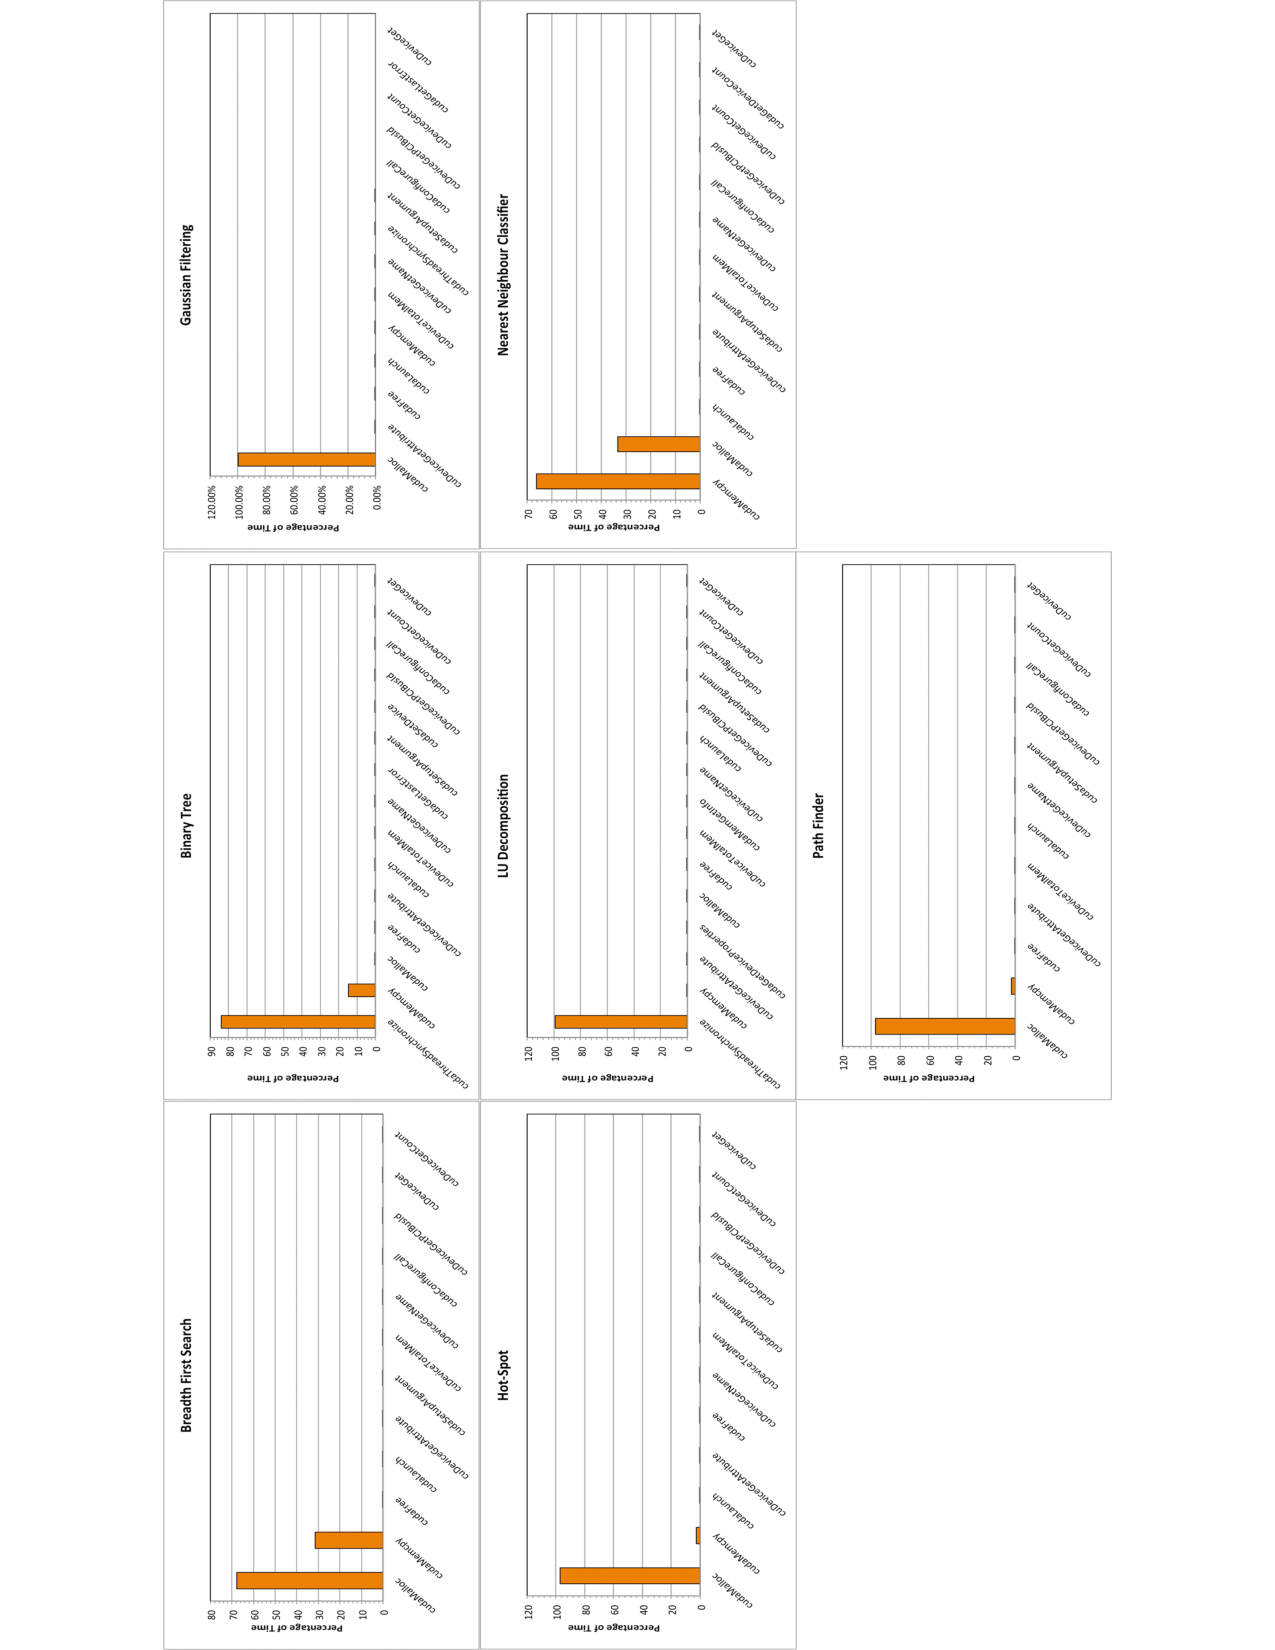
\includegraphics[scale=0.6]{../imgs/x630.pdf}
\caption{testing}
\label{??}
\end{figure*}




\newpage
\section{Benchmarking using a GeForce GTX 650}
These tests have been performed using a GeForce GTX 650 and hardware platform 2 specified in Table \ref{table2}. The below figures depict the time take for each individual API call for all seven test cases.

\begin{figure*}[!h]
\centering
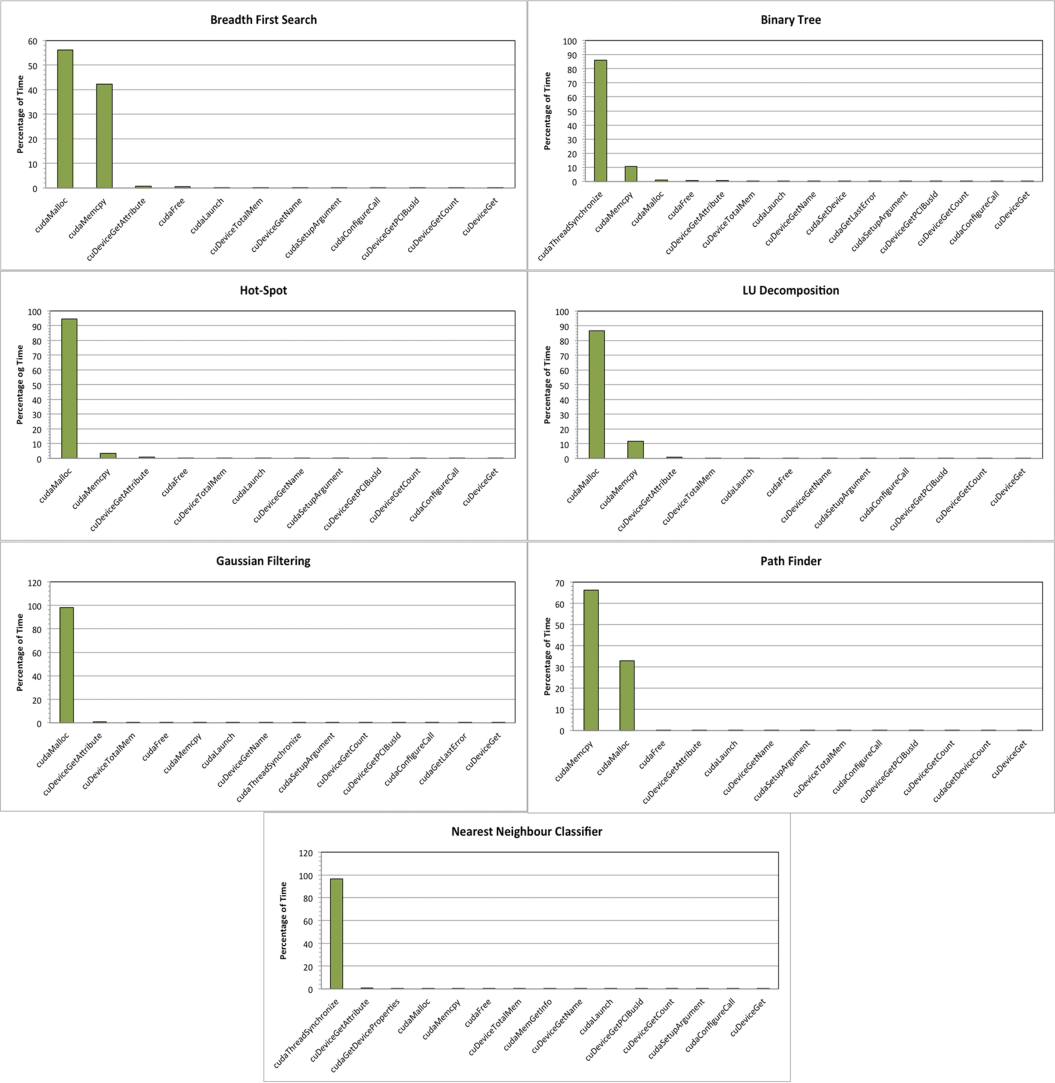
\includegraphics[scale=0.6]{../imgs/x650.pdf}
\caption{testing}
\label{??}
\end{figure*}




\newpage
\section{Benchmarking using a Quadro 6000}
These tests have been performed using a Quadro 6000 and hardware platform 3 specified in the table in Table \ref{table2}. The below figures depict the time take for each individual API call for all seven test cases.

\begin{figure*}[!h]
\centering
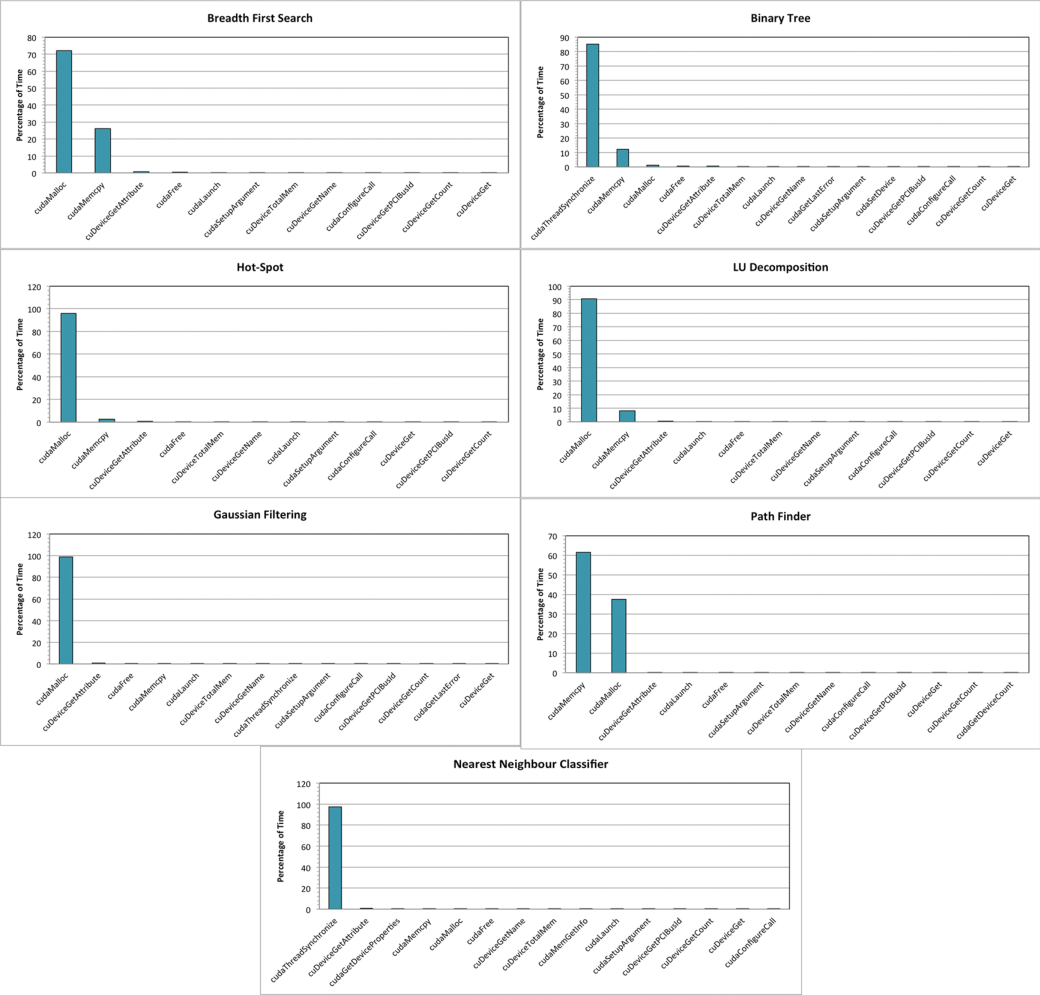
\includegraphics[scale=0.6]{../imgs/m6000.pdf}
\caption{testing}
\label{??}
\end{figure*}






\newpage
\section{Results}

The below figures summarizes all the results from all three different NVIDIA GPU's. 


\begin{figure*}[!h]
\centering
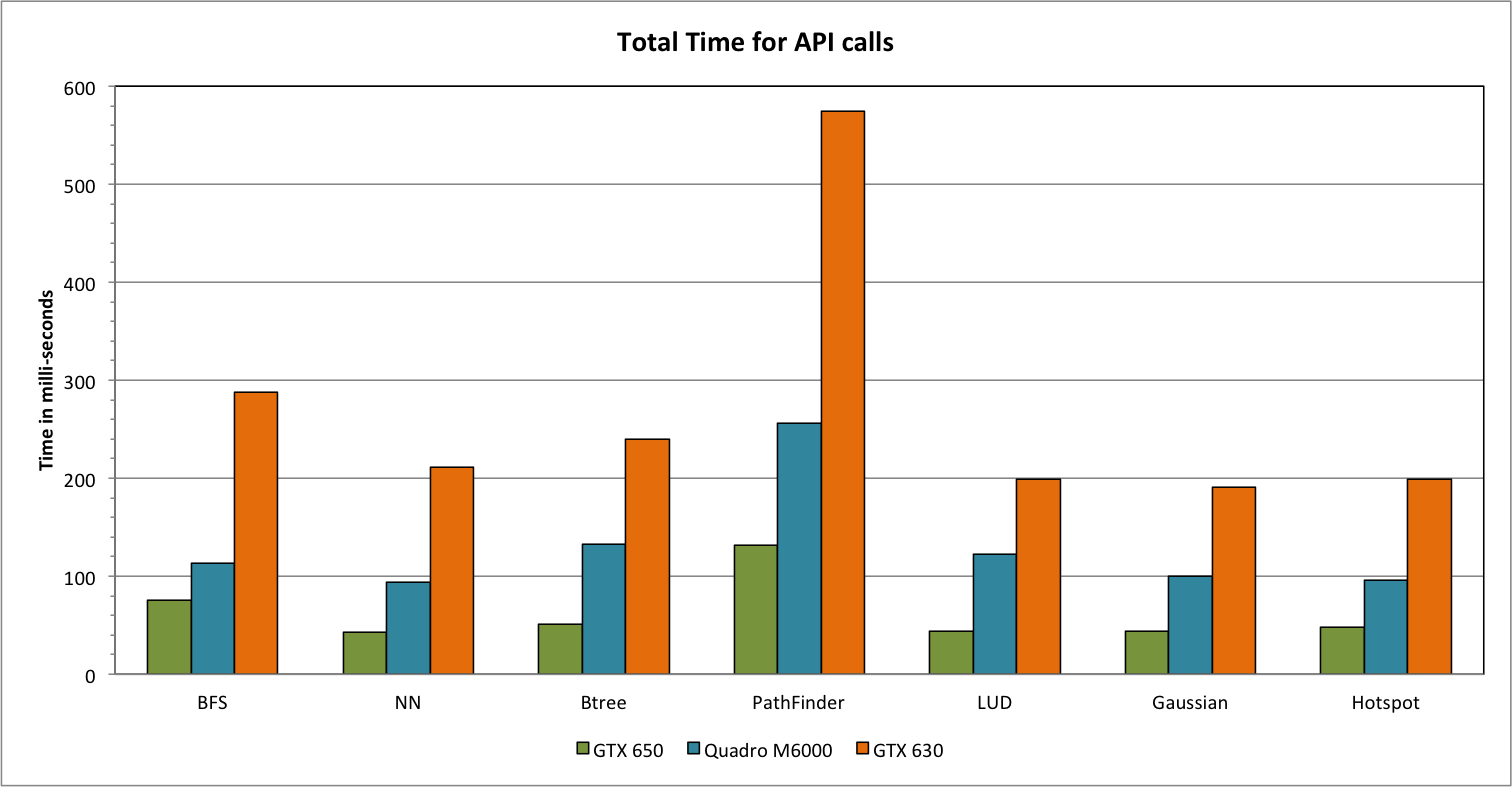
\includegraphics[width=0.95\textwidth,height=8cm]{../imgs/api_calls.png}
\caption{testing}
\label{??}
\end{figure*}

\begin{figure*}[!h]
\centering
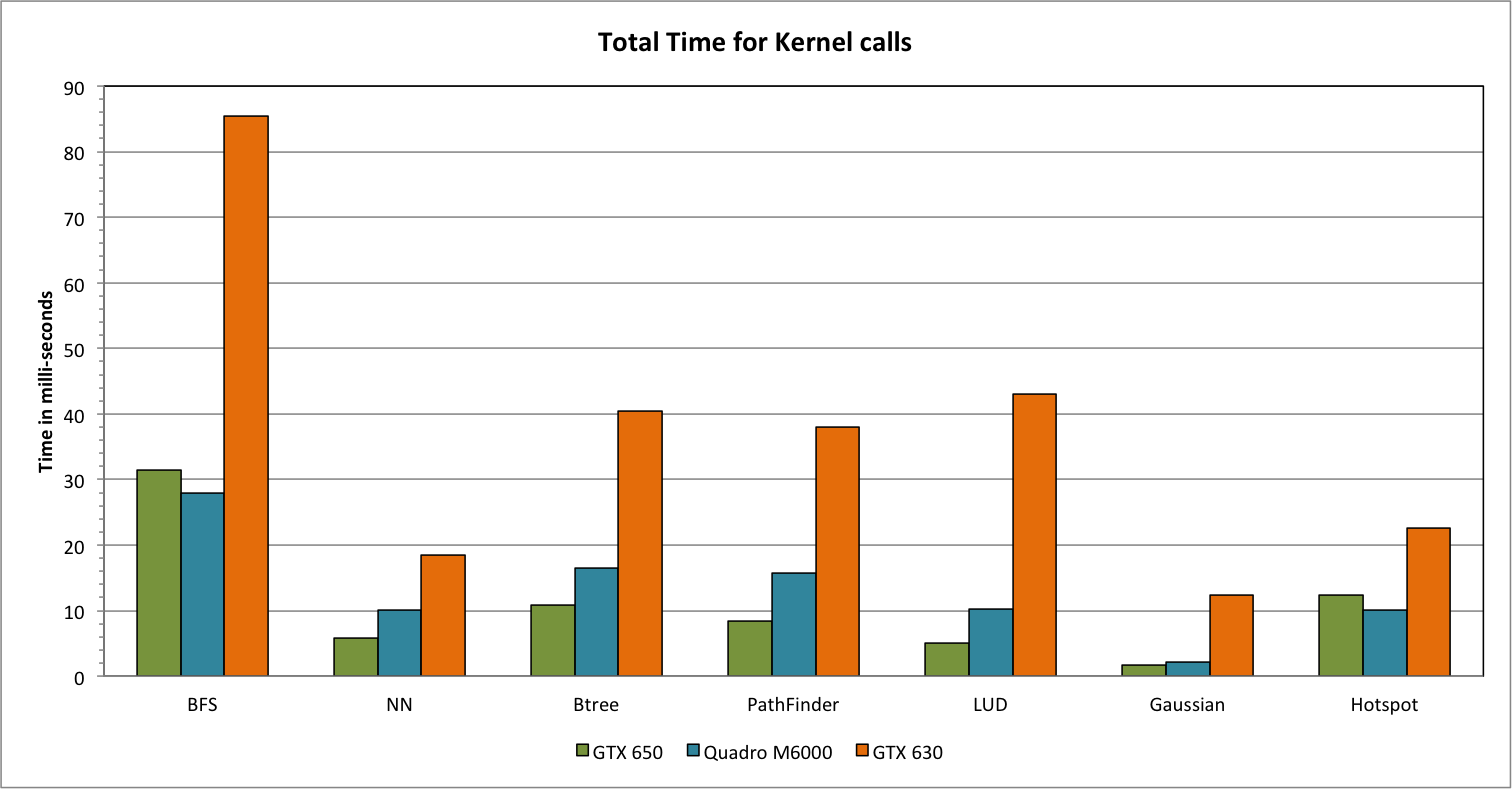
\includegraphics[width=0.95\textwidth,height=8cm]{../imgs/kernel_calls.png}
\caption{testing}
\label{??}
\end{figure*}

\begin{figure*}[!h]
\centering
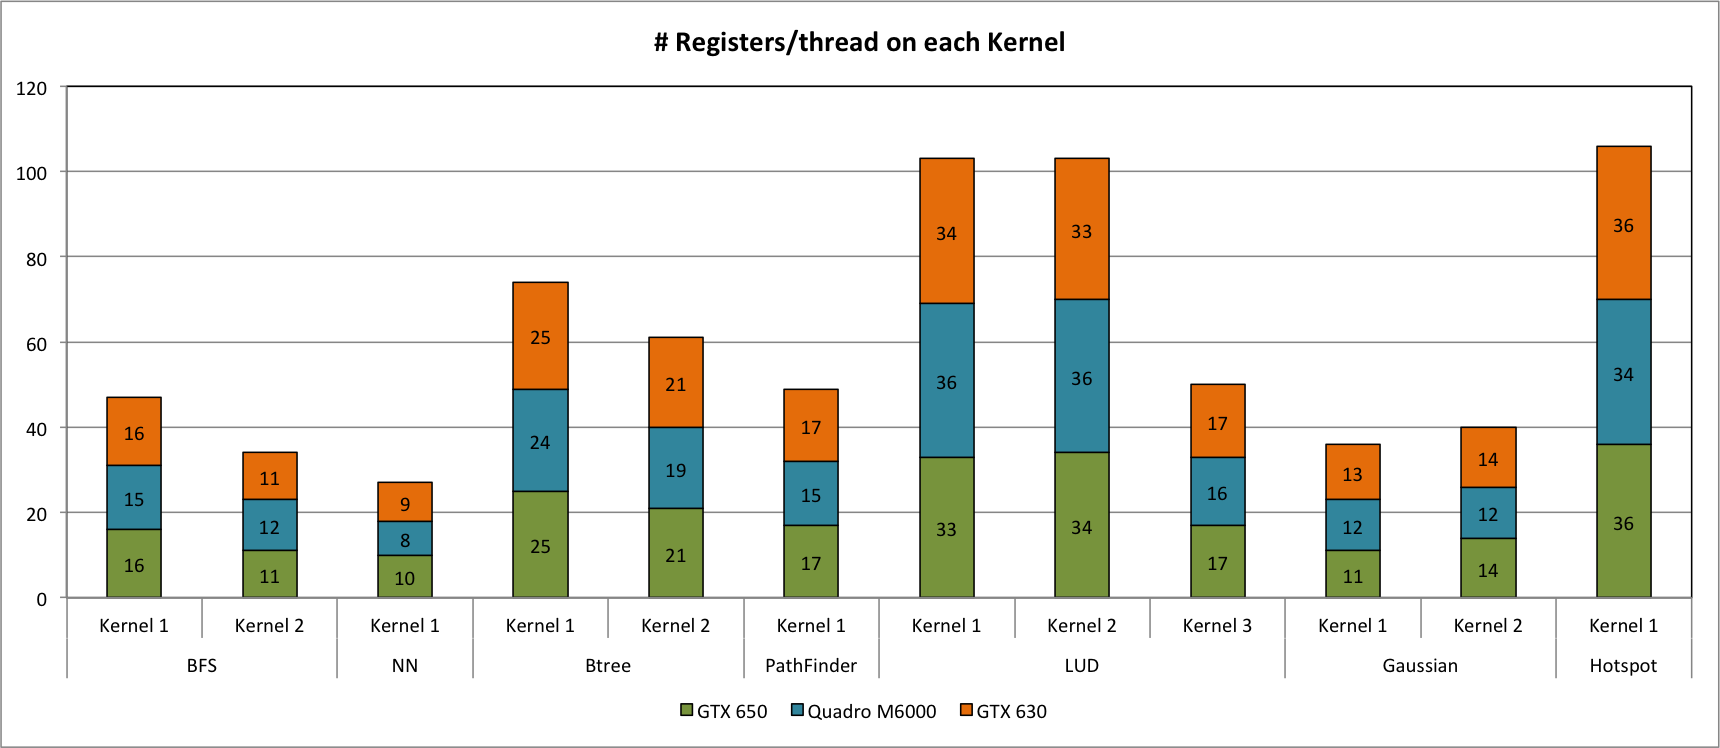
\includegraphics[width=0.95\textwidth,height=6cm]{../imgs/register_thread.png}
\caption{testing}
\label{??}
\end{figure*}

\begin{figure*}[!h]
\centering
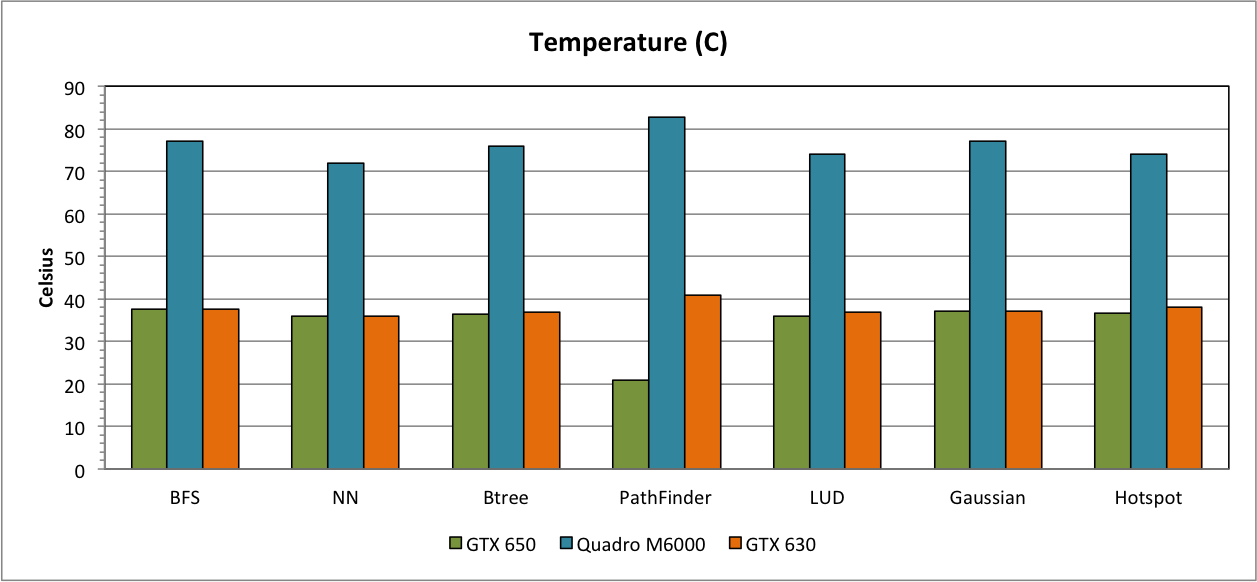
\includegraphics[width=0.95\textwidth,height=6cm]{../imgs/temp.png}
\caption{testing}
\label{??}
\end{figure*}

\begin{figure*}[!h]
\centering
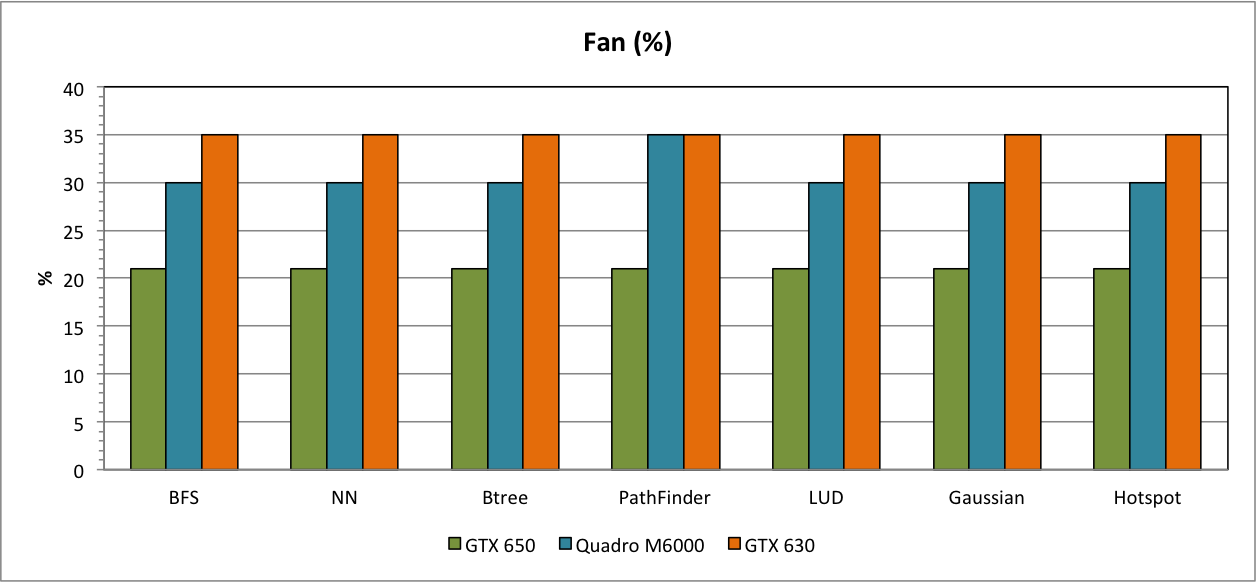
\includegraphics[width=0.95\textwidth,height=6cm]{../imgs/fan.png}
\caption{testing}
\label{??}
\end{figure*}




\newpage
\section{Analysis}
.......


\newpage
\section{Conclusion}

Though the test cases ran for several seconds ..if they ran for minutes the differences will be even more profound


\end{document}
